\documentclass[10pt]{article}
\usepackage[margin=15mm]{geometry}
\usepackage{amsmath,amssymb,tikz,pgfplots}
\pgfplotsset{compat=1.18}
\definecolor{digitZero}{HTML}{246C91}
\definecolor{digitOne}{HTML}{BC632E}
\pagestyle{empty}
\begin{document}
\begin{center}
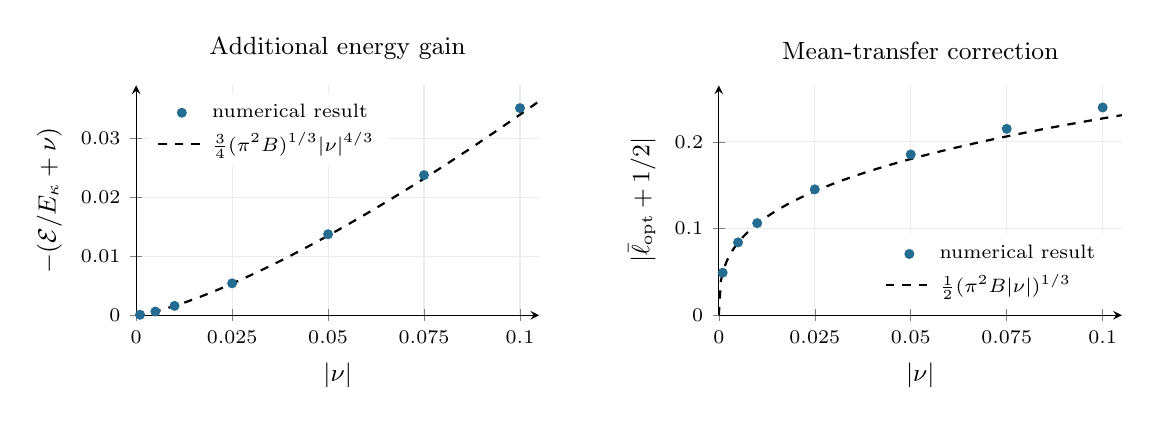
\begin{tikzpicture}
\begin{axis}[width=6.7cm,height=4.5cm,scale only axis=false,
 axis lines=left,tick label style={font=\scriptsize},label style={font=\small},
 title style={font=\small},legend style={font=\scriptsize,draw=none,fill=white},
 legend cell align=left,scaled ticks=false,grid=major,grid style={gray!15},
 tick label style={/pgf/number format/use period,/pgf/number format/fixed,/pgf/number format/precision=3,font=\scriptsize},xmin=0,xmax=.105,ymin=0,ymax=.039,
 xlabel={$|\nu|$},ylabel={$-(\mathcal E/E_\kappa+\nu)$},
 title={Additional energy gain},
 xtick={0,.025,.05,.075,.1},ytick={0,.01,.02,.03},legend pos=north west]
\addplot[only marks,mark=*,mark size=1.6pt,digitZero] coordinates {(0.001,7.33983740395e-05) (0.005,0.000628652698002) (0.01,0.00158712484089) (0.025,0.00541166475888) (0.05,0.0137410457162) (0.075,0.0237707757236) (0.1,0.0351443959674)};
\addlegendentry{numerical result}
\addplot[black,dashed,thick,domain=0:.105,samples=101] {.75*(pi^2*(.5-4/pi^2))^(1/3)*x^(4/3)};
\addlegendentry{$\frac34(\pi^2B)^{1/3}|\nu|^{4/3}$}
\end{axis}
\begin{axis}[width=6.7cm,height=4.5cm,scale only axis=false,
 axis lines=left,tick label style={font=\scriptsize},label style={font=\small},
 title style={font=\small},legend style={font=\scriptsize,draw=none,fill=white},
 legend cell align=left,scaled ticks=false,grid=major,grid style={gray!15},
 tick label style={/pgf/number format/use period,/pgf/number format/fixed,/pgf/number format/precision=3,font=\scriptsize},at={(7.4cm,0)},anchor=south west,
 xmin=0,xmax=.105,ymin=0,ymax=.265,xlabel={$|\nu|$},ylabel={$|\bar\ell_{\rm opt}+1/2|$},
 title={Mean-transfer correction},
 xtick={0,.025,.05,.075,.1},ytick={0,.1,.2},legend pos=south east]
\addplot[only marks,mark=*,mark size=1.6pt,digitZero] coordinates {(0.001,0.0489886332667) (0.005,0.0839468359711) (0.01,0.106218464559) (0.025,0.14511718918) (0.05,0.185378303053) (0.075,0.21489665688) (0.1,0.239551285836)};
\addlegendentry{numerical result}
\addplot[black,dashed,thick,domain=0:.105,samples=201] {.5*(pi^2*(.5-4/pi^2)*x)^(1/3)};
\addlegendentry{$\frac12(\pi^2B|\nu|)^{1/3}$}
\end{axis}
\end{tikzpicture}
\end{center}\end{document}
